% Template for ICASSP-2016 paper; to be used with:
%          spconf.sty  - ICASSP/ICIP LaTeX style file, and
%          IEEEbib.bst - IEEE bibliography style file.
% --------------------------------------------------------------------------
\documentclass{article}
\usepackage{spconf,amsmath,graphicx}

% Example definitions.
% --------------------
\def\x{{\mathbf x}}
\def\L{{\cal L}}

% Title.
% ------
\title{HYBRID MUSIC RECOMMENDER USING CONTENT-BASED AND SOCIAL INFORMATION}
%
% Single address.
% ---------------
\name{Paulo Chiliguano, Gyorgy Fazekas}%\thanks{Thanks to XYZ agency for funding.}}
\address{Queen Mary, University of London\\School of Electronic Engineering and Computer Science\\Mile End Road, London E1 4NS, UK}
%
% For example:
% ------------
%\address{School\\
%	Department\\
%	Address}
%
% Two addresses (uncomment and modify for two-address case).
% ----------------------------------------------------------
%\twoauthors
%  {A. Author-one, B. Author-two\sthanks{Thanks to XYZ agency for funding.}}
%	{School A-B\\
%	Department A-B\\
%	Address A-B}
%  {C. Author-three, D. Author-four\sthanks{The fourth author performed the work
%	while at ...}}
%	{School C-D\\
%	Department C-D\\
%	Address C-D}
%
\begin{document}
%\ninept
%
\maketitle
%
\begin{abstract}
Internet resources available today, including songs, albums, playlists or podcasts, that a user cannot discover require a tool for filtering the items that a user might consider relevant. Several recommendation techniques have been developed since the Internet explosion to achieve this filtering task. In an attempt to recommend relevant songs to users, we propose an hybrid music recommender system that considers real-world users information and high-level representation for audio data. The system uses a convolutional deep neural network to represent audio segments by genre and uses estimation of distribution algorithms to represent the user listening behavior. Finally, content-based filtering is employed to generate Top-N recommendations. Our proposed hybrid music recommender presents a convincing performance improvement over the  content-based baseline model.
\end{abstract}
%
\begin{keywords}
	Deep Learning, Convolutional Neural Networks, Estimation of Distribution Algorithms, Recommender Systems, MIR.

\end{keywords}
%
\section{Introduction}
\label{sec:intro}

Recommender systems~\cite{melville2010recommender} are software or technical facilities to provide items suggestions or predict customer preferences by using prior user information. These systems play an important role in commercial applications to increase sales and improve user satisfaction. In general, recommender systems can be categorized in two major groups: collaborative filtering (CF) and content-based (CB) filtering. In CF~\cite{Yao2015453, Burke2002331}, a \emph{m$\times$n} rating matrix represents the relationships between \textit{m} users and \textit{n} items and recommendations are based on the computed similarities between rows (for users) or columns (for items). CF can be further subdivided in neighborhood models~\cite{Hu2008263}. The recommendation process in CF is independent of the item features. However, CF ignores the items in the \textit{long tail}~\cite{Yin2012896} and it is unable to handle the \textit{cold-start}~\cite{Dai20141760} problem. On the other hand, CB filtering~\cite{Lops2011} is based on the analysis of the features that describe the items. The recommendation component consists in matching up the attributes of the items that a user has already rated, usually referred as the \textit{user profile}, against the attributes of a previously unseen products to produce a list of \emph{top-N} recommendations. The recommendation process in CB is entirely based on the attributes of the items, thus, the recommendations produced for each user is independent from the other users. Also, a CB recommender allows to recommend items that do not have any rating, therefore, the effects of cold-start problem can be diminished. However, the quality of recommendations from CB techniques depends on the size of historical dataset. A hybrid recommender~\cite{Burke2002331} system is usually developed through the combination of CF and CB recommendation techniques to boost the advantages of CF by considering the feedback (rating) of users and the advantages of CB by taking into count the item attributes. Methods of combining recommendation techniques to accomplish hybridization can be classified in weighted, switching, mixed, feature combination, cascade, feature augmentation and meta-level methods.

In Section~\ref{sec:background}, we revise related work in music recommender systems. In Section~\ref{sec:format}, we present our proposed hybrid recommendation approach and its stages, also we describe the music genre representation of audio and user profile modeling. In Section~\ref{sec:pagestyle}, we present the experiments and evaluation protocols to assess the performance of the hybrid recommender. In Section~\ref{sec:typestyle}, we discuss and analyze the results from the conducted experiments to evaluate the proposed hybrid music recommender.  We conclude in Section~\ref{sec:refs}, we present the conclusions and some thoughts for further research.


\section{Background}
\label{sec:background}

A hybrid music recommender system proposed by~\cite{Yoshii2008435} considered the rating scores collected from Amazon.co.jp and acoustic features derived from the signals of musical pieces corresponding to Japanese CD singles that were ranked in weekly top-20 from April 2000 to December 2005. Acoustic features for each piece are represented as a \textit{bag-of-timbres}, i.e., a set of weights of polyphonic timbres, equivalent to a 13-dimensional MFCC representation. Bags of timbres are computed with a Gaussian Mixture Model, considering the same combination of Gaussians for every musical piece. A music recommender proposed by~\cite{NIPS2013_5004} use a latent factor model for CB recommendation and the implementation of a convolutional neural network (CNN)~\cite{Bengio-et-al-2015-Book} to predict the latent factors from music audio. To obtain 50-dimension latent vectors, they used a weighted matrix factorization (WMF) algorithm on the Taste Profile Subset~\cite{Bertin-Mahieux2011}. Also, they retrieved audio clips for over 99\% of the songs in the dataset from 7digital.com. To train the CNN, the latent vectors obtained through the WMF are used as ground truth. The input of the CNN is a log-compressed mel-spectrogram with 128 components computed from windows of 1,024 samples and a hop size of 512 samples (sampling rate of 22,050 Hz) of a 3 seconds window sampled randomly for each audio clip. They used 10-fold cross validation and obtained an average area under the ROC curve (AUC) of 0.86703 for prediction based on the latent factor vectors, outperforming the bag-of-timbres approach.

Inspired by natural selection of species, estimation of distribution algorithms (EDAs)~\cite{pelikan2015estimation, Ding2015451, Santana:Bielza:Larrañaga:Lozano:Echegoyen:Mendiburu:Armañanzas:Shakya:2009:JSSOBK:v35i07} are optimization techniques that estimate a probabilistic model from a sample of promising individuals. The sample is used to generate a new population that satisfy a criteria, i.e., minimization of a \textit{fitness} function. In Figure~\ref{fig:eda}, we show the general flowchart of an EDA. Regarding to the types of distributions that an EDA are able to capture can be categorized in four broad groups: discrete variables EDA, permutation EDA, real-valued vectors EDA and genetic programming EDA.

In this paper, we present a hybrid music recommender to mitigate the cold-start problem in recommendation strategies. First, we use CNNs to describe the time-frequency content of an audio clip with a n-dimensional vector, whose dimensions represent the probability of a clip to belong to an specific music genre. Second, as a primary contribution, EDAs are investigated to model user profiles in terms of probabilities of music genres preferences. The algorithms use play count and the content vector of each song in the user's collection to optimize the profile. To our knowledge, this is the first approach that uses a continuous EDA for user profile modeling in recommender systems.

\begin{figure}[htb]
	
	\begin{minipage}[b]{1.0\linewidth}
		\centering
		\centerline{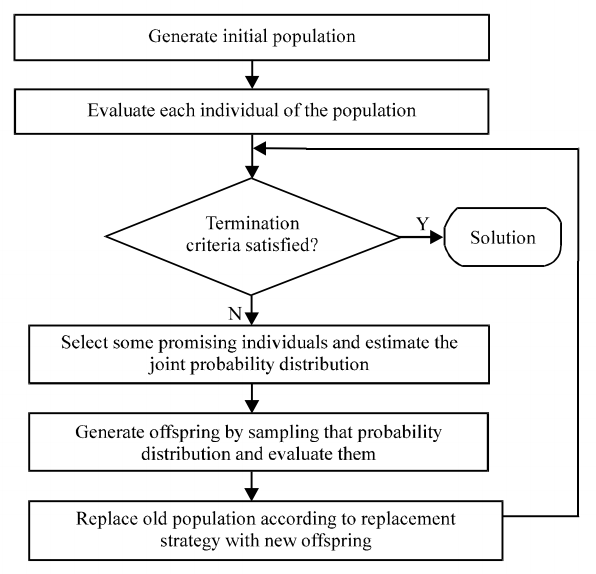
\includegraphics[width=8.5cm]{eda.png}}
		%  \vspace{2.0cm}
		%\centerline{(a) Result 1}\medskip
	\end{minipage}
	%
	\caption{Flowchart of an EDA presented in~\cite{Ding2015451}}
	\label{fig:eda}
	%
\end{figure}



\section{METHODOLOGY}
\label{sec:format}

The methodology used to develop our hybrid music recommender, shown in Figure~\ref{fig:hybrid} consists of four main stages. First, the collection of real world user-item data corresponding to the play counts of specific songs and the fetching of audio clips of the unique identified songs in the dataset. Secondly, the implementation of the CNN to represent the audio clips in terms of music genre probabilities as n-dimensional vectors. Next, permutation EDA and a continuous EDA are investigated to model user profiles based on the rated songs above a threshold. Finally, the process of top-N recommendation for the baseline and the hybrid recommender is described.

\begin{figure}[htb]
	
	\begin{minipage}[b]{1.0\linewidth}
		\centering
		\centerline{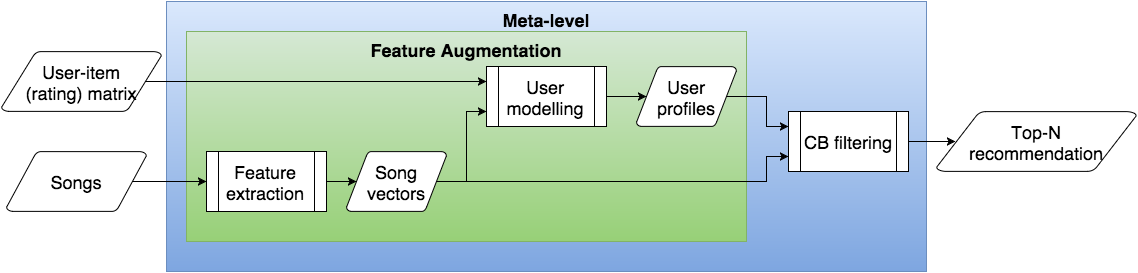
\includegraphics[width=8.5cm]{hybrid.png}}
		%  \vspace{2.0cm}
		%\centerline{(a) Result 1}\medskip
	\end{minipage}
	%
	\caption{Diagram of hybrid music recommender}
	\label{fig:hybrid}
	%
\end{figure}

\subsection{Data collection}
The Million Song Dataset~\cite{Bertin-Mahieux2011} is a collection of audio features and metadata for a million contemporary popular music tracks which provides ground truth for evaluation research in Music Information Retrieval (MIR). This collection is also complemented by the Taste Profile subset which provides 48,373,586 triplets, each of them consist of anonymous user ID, Echo Nest song ID and play count. We choose this dataset because it is publicly available and it contains enough data for user modeling and recommender evaluation. However, it has potential mismatches between song ID and metadata, thus, we filter the triplets without errors in song IDs, obtaining 45,795,100 triplets. In addition, we reduce significantly the size of the dataset for experimental purposes and we consider only the users with more than 1,000 played songs and select the song identifiers of 1,500 most played songs. At the end, we obtain 65,327 triplets. For each song ID of the 1,500 most played songs, we retrieve the Echo Nest track ID and preview URL to fetch audio data from 7digital, resulting in a total of 640 available MP3 clips with a duration of 30 to 60 seconds (44.1 kHz, 128 kbps, stereo).

The reduced taste profile dataset represent the user listening habits as implicit feedback, i.e., play counts of songs, it is necessary to normalize the listening habits as explicit feedback, i.e., range of values $[1\ldots5]$ that indicate how much a user likes a song. Normalization of play counts is computed with the complementary cumulative distribution of play counts of a user, following the procedure given by~\cite{1242}.

\subsection{Probability of music genre representation}

Following the steps of~\cite{NIPS2013_5004}, a segment equivalent to 3 seconds of each audio clip is loaded at a sampling rate of 22,050 Hz and converted to mono channel. For every segment, a mel-scaled power spectrogram with 128 bands is computed from windows of 1,024 samples with a hop size of 512 samples, resulting in a spectrogram of 130 frames with 128 components. Next, the spectrogram is converted to logarithmic scale in dB using peak power as reference. The spectrograms are normalized to have zero mean and unit variance in each frequency band. We use the GTZAN dataset~\cite{Tzanetakis2002293} as ground truth for training, validation and testing the CNN.

In our project, we recreate a similar CNN architecture for music genre classification in~\cite{DBLP:journals/corr/KereliukSL15}. A batch size of 20 and a dropout rate of 0.20 for the convolutional layer units are considered. The reshape of the spectrograms (130 frames$\times$128 frequency bands) to a 4-dimension tensor, compatible with the input of the first convolutional layer (batch size$\times$1$\times$130$\times$128), is required. The first convolutional layer consists of 32 filters, each one with a size of 8 frames, with a max-pooling downsampling of 4, to reduce the size of the spectrogram along the time axis. The size of the resulting spectrogram is 30$\times$128 and the output of this first convolutional layer is a 4-dimension tensor with a size of 20$\times$32$\times$30$\times$128. The second convolutional layer consists of 32 filters, each one with a size of 8 frames, with a max-pooling downsampling of 4, to reduce the size of the spectrogram obtained in the first layer. The size of the new spectrogram is 5$\times$128 and the output of this second convolutional layer is a 4-dimension tensor with a size of 20$\times$32$\times$5$\times$128. Following the convolution process, the reshape of the 4-dimensional tensor of the output of the second convolutional layer is required to feed the fully connected multi-layer perceptron (MLP). The MLP consists of 500 ReLUs. Finally, the classification of music genre is accomplished with a logistic regression layer with 10 softmax units. Each output value corresponds to a music genre and each value represents the probability of a song to belong to a specific music genre.

%n the particular case for the time-frequency representation of each audio clip in the GTZAN dataset, we generate a list of the genre associated to each audio fragment that represent the target values (ground truth). This procedure for the GTZAN dataset is repeated for 9 times, considering the rest of 3-seconds fragments in each audio clip of the dataset for training, validation and testing of the CDNN

%In our approach, we describe the songs in terms of n-dimensional vectors. Each dimension in the vector represent the probability of the song to belong to a music genre. The probability estimation is obtained from a music classifier implemented with a deep learning technique. 

\subsection{User profile modeling with EDAs}

In our project, we model each user profile following the EDA approach of~\cite{Liang2014781} by minimizing a fitness function given by Equation~\eqref{eq:fitness}
\
\begin{equation}
fitness(profile_u) =\sum_{i\in S_u}\log(r_{u,i}\times sim(profile_u,t_i))
\label{eq:fitness}
\end{equation}
where \emph{$sim(profile_u,t_i)$} is the cosine similarity between the profile of user \emph{u} and the vector of probabilities of the song \emph{i}, which is in the subset of relevant songs \emph{$S_u$}, and \emph{$r_{u,i}$} is the rating of song \emph{i} given by user \emph{u}. In this approach, the probability values are discretized in 50 evenly spaced values over the interval $[0.1, 0.9]$.

Moreover, we extended the EDA approach using the continuous univariate marginal distribution algorithm $UMDA_c^G$ of~\cite{gallagher2007bayesian}.

\subsection{Top-N songs recommendation}

In our hybrid music model, the CB filtering module computes the similarity between a user interest profile and a each song vector in the test set. The songs are ranked in descending order and the first $N$ songs of this list are recommended.

\section{EXPERIMENTS}
\label{sec:pagestyle}
The hybrid music recommender system proposed in this project is evaluated through an off-line experiment and the results are presented with decision based metrics: Precision, recall, F1 measure and accuracy~\cite{1242}.

The reduced taste profile dataset is split in a training and a test set. For each user in the dataset, a random sample corresponding to 20 \% of the total number of ratings is assigned to the test set, and the rest 80 \% is assigned to the training set. The split process is iterated for 10 times, resulting in a total of 10 training and 10 test sets.

\subsection{Top-N evaluation}
For each song in the user test set, we look up if the song is included or not in the top-N recommendations. If the song rating is above the threshold (we find a rating $\geq$ 3 out of 5 suitable) and the song is ranked in the top-N recommendations, we count as a true positive, otherwise, if the song is not included in the recommendations we count as false negative. On the other hand, if the song rating is below the threshold and the song appears in the top-N recommendations, we count as a false positive, otherwise, if the song is not included on the recommendations, we count as a false negative.

%The paper title (on the first page) should begin 1.38 inches (35 mm) from the
%top edge of the page, centered, completely capitalized, and in Times 14-point,
%boldface type.  The authors' name(s) and affiliation(s) appear below the title
%in capital and lower case letters.  Papers with multiple authors and
%affiliations may require two or more lines for this information. Please note
%that papers should not be submitted blind; include the authors' names on the
%PDF.

\section{RESULTS}
\label{sec:typestyle}
In general, the results of the top-N evaluation demonstrate that the hybrid music recommender based on a permutation EDA presents a better performance compared with both the CB recommender and the hybrid approach based on a continuous EDA. In Table~\ref{table:recn5}, the results of top-5 recommendation are shown.
\begin{table}[htb]
	\resizebox{0.6\linewidth}{!}{\centering % used for centering table
	\begin{minipage}[b]{1.0\linewidth}
		\begin{tabular}{c c c c c} % centered columns (4 columns)
			\hline\hline %inserts double horizontal lines
			Recommender & Precision & Recall & F1 & Accuracy \\ [0.5ex] % inserts table
			%heading
			\hline % inserts single horizontal line
			Content-based (baseline) & 0.275 $\pm$ 0.087 & 0.010 $\pm$ 0.003 & 0.020 $\pm$ 0.007 & 0.681 $\pm$ 0.008 \\ % inserting body of the table
			Hybrid (permutation EDA) & \textbf{0.391 $\pm$ 0.182} & \textbf{0.013 $\pm$ 0.007} & \textbf{0.025 $\pm$ 0.013} & \textbf{0.685 $\pm$ 0.009} \\
			Hybrid (continuous UMDA) & 0.318 $\pm$ 0.142 & 0.011 $\pm$ 0.005 & 0.021 $\pm$ 0.011 & 0.683 $\pm$ 0.009 \\ [1ex] % [1ex] adds vertical space
			\hline %inserts single line
		\end{tabular}
	\end{minipage}}
	
	\caption{Evaluation of recommender systems (N=5)} % title of Table
	\label{table:recn5} % is used to refer this table in the text
\end{table}

In Table~\ref{table:recn10}, the results of top-10 songs recommendation are shown. In this case, the precision value improves for the CB recommender. The accuracy values for all recommender systems tend to decrease.
\begin{table}[htb]
	\resizebox{0.6\linewidth}{!}{\centering % used for centering table
	\begin{minipage}[b]{1.0\linewidth}
		\begin{tabular}{c c c c c} % centered columns (4 columns)
			\hline\hline %inserts double horizontal lines
			Recommender & Precision & Recall & F1 & Accuracy \\ [0.5ex] % inserts table
			%heading
			\hline % inserts single horizontal line
			Content-based (baseline) & 0.301 $\pm$ 0.059 & 0.022 $\pm$ 0.007 & 0.041 $\pm$ 0.012 & 0.678 $\pm$ 0.007 \\ % inserting body of the table
			Hybrid (permutation EDA) & \textbf{0.370 $\pm$ 0.073} & \textbf{0.024 $\pm$ 0.007} & \textbf{0.045 $\pm$ 0.013} & \textbf{0.682 $\pm$ 0.009} \\
			Hybrid (continuous UMDA) & 0.309 $\pm$ 0.100 & 0.019 $\pm$ 0.007 & 0.036 $\pm$ 0.013 & 0.679 $\pm$ 0.009 \\ [1ex] % [1ex] adds vertical space
			\hline %inserts single line
		\end{tabular}
	\end{minipage}}
	
	\caption{Evaluation of recommender systems (N=10)} % title of Table
	\label{table:recn10} % is used to refer this table in the text
\end{table}

In Table~\ref{table:recn20}, the results of top-20 songs recommendation are shown. In this case, the recall values rise for all the recommender systems, compared with the top-5 and top-10 recommendations, but the precision and accuracy tend to decrease. At this point, we can deduce that our hybrid recommender approaches could improve the recall without losing reached precision if $N$ is in a value between 10 and 20.
\begin{table}[htb]
	\resizebox{0.6\linewidth}{!}{\centering % used for centering table
	\begin{minipage}[b]{1.0\linewidth}
		\begin{tabular}{c c c c c} % centered columns (4 columns)
			\hline\hline %inserts double horizontal lines
			Recommender & Precision & Recall & F1 & Accuracy \\ [0.5ex] % inserts table
			%heading
			\hline % inserts single horizontal line
			Content-based (baseline) & 0.281 $\pm$ 0.052 & 0.041 $\pm$ 0.006 & 0.071 $\pm$ 0.010 & 0.666 $\pm$ 0.006 \\ % inserting body of the table
			Hybrid (permutation EDA) & \textbf{0.363 $\pm$ 0.041} & \textbf{0.047 $\pm$ 0.008} & \textbf{0.084 $\pm$ 0.014} & \textbf{0.676 ±  $\pm$ 0.007} \\
			Hybrid (continuous UMDA) & 0.302 $\pm$ 0.067 & 0.039 $\pm$ 0.011 & 0.070 $\pm$ 0.019 & 0.671 $\pm$ 0.010 \\ [1ex] % [1ex] adds vertical space
			\hline %inserts single line
		\end{tabular}
	\end{minipage}}
	
	\caption{Evaluation of recommender systems (N=20)} % title of Table
	\label{table:recn20} % is used to refer this table in the text
\end{table}

%To achieve the best rendering both in printed proceedings and electronic proceedings, we
%strongly encourage you to use Times-Roman font.  In addition, this will give
%the proceedings a more uniform look.  Use a font that is no smaller than nine
%point type throughout the paper, including figure captions.

%In nine point type font, capital letters are 2 mm high.  {\bf If you use the
%smallest point size, there should be no more than 3.2 lines/cm (8 lines/inch)
%vertically.}  This is a minimum spacing; 2.75 lines/cm (7 lines/inch) will make
%the paper much more readable.  Larger type sizes require correspondingly larger
%vertical spacing.  Please do not double-space your paper.  TrueType or
%Postscript Type 1 fonts are preferred.

%The first paragraph in each section should not be indented, but all the
%following paragraphs within the section should be indented as these paragraphs
%demonstrate.


% Below is an example of how to insert images. Delete the ``\vspace'' line,
% uncomment the preceding line ``\centerline...'' and replace ``imageX.ps''
% with a suitable PostScript file name.
% -------------------------------------------------------------------------
%\begin{figure}[htb]

%\begin{minipage}[b]{1.0\linewidth}
  %\centering
  %\centerline{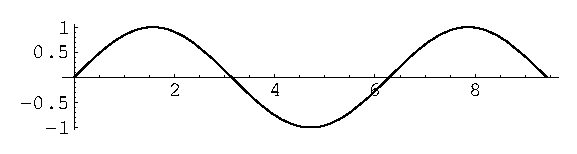
\includegraphics[width=8.5cm]{image1}}
%  \vspace{2.0cm}
  %\centerline{(a) Result 1}\medskip
%\end{minipage}
%
%\begin{minipage}[b]{.48\linewidth}
  %\centering
  %\centerline{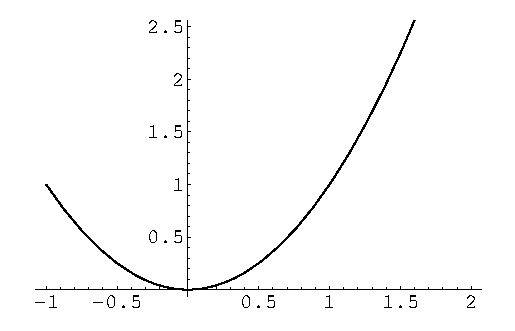
\includegraphics[width=4.0cm]{image3}}
%  \vspace{1.5cm}
  %\centerline{(b) Results 3}\medskip
%\end{minipage}
%\hfill
%\begin{minipage}[b]{0.48\linewidth}
  %\centering
  %\centerline{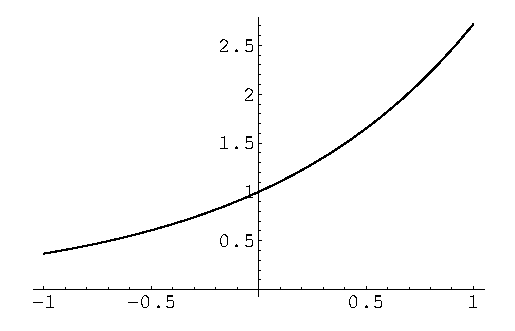
\includegraphics[width=4.0cm]{image4}}
%  \vspace{1.5cm}
  %\centerline{(c) Result 4}\medskip
%\end{minipage}
%
%\caption{Example of placing a figure with experimental results.}
%\label{fig:res}
%
%\end{figure}

\section{CONCLUSIONS AND FURTHER WORK}
\label{sec:refs}
The whole aim of our project has been the design and the implementation of an hybrid music recommender in order to mitigate the cold-start problem in content-based recommender systems. We investigated several types of hybridization in recommender systems to choose a suitable architecture for the available datasets. To represent real world users and raw waveforms, we decided to investigate and implement state-of-the-art techniques. Despite of the success in computer vision field, we found in our project that convolutional deep neural networks achieve similar results to a long-established content-based music genre classifier in music information retrieval field. Due to the natural selection concept associated to estimation of distribution algorithms, we investigated and considered these optimization techniques for modeling users' listening behavior in terms of probabilities of music genres from the songs they have listened. On the other hand, we found that a limited number of genres for song representation lead us to coarse predictions according to decision-based metrics.

For the future, we have the intention to enhance our hybrid music recommender considering a wide range of music genres or latent vectors for item representation. We shall work on investigating several configurations of convolutional deep neural networks and different types of deep learning techniques, particularly, unsupervised learning approaches, for a better high-level representation of audio waveforms. In addition, we will continue investigating the fascinating estimation of distribution algorithms, considering another optimization functions, to model user profiles in recommender systems. Finally, we also consider the evaluation of the hybrid recommender with an online experiment.
%List and number all bibliographical references at the end of the
%paper. The references can be numbered in alphabetic order or in
%order of appearance in the document. When referring to them in
%the text, type the corresponding reference number in square
%brackets as shown at the end of this sentence \cite{C2}. An
%additional final page (the fifth page, in most cases) is
%allowed, but must contain only references to the prior
%literature.

%\vfill\pagebreak

% References should be produced using the bibtex program from suitable
% BiBTeX files (here: strings, refs, manuals). The IEEEbib.bst bibliography
% style file from IEEE produces unsorted bibliography list.
% -------------------------------------------------------------------------
\bibliographystyle{IEEEbib}
\bibliography{strings,refs}

\end{document}
